% =========================================================================
%  Can Pink Elephants Exist — Mid-Submission Report (ACL Format)
% =========================================================================
\documentclass[11pt]{article}
\usepackage{../acl-style-files/acl}
\usepackage{times}
\usepackage{latexsym}
\usepackage[T1]{fontenc}
\usepackage[utf8]{inputenc}
\usepackage{microtype}
\usepackage{graphicx}
\usepackage{amsmath,amssymb}
\usepackage{booktabs}
\usepackage{hyperref}
\usepackage{xcolor}

\setlength\titlebox{6cm}

\title{Can Pink Elephants Exist:\\Mapping the Logic--Memory Conflict in LLMs}

\author{
  Eashaan Thakur \and Hemang Joshi \and Naman Singhal \\
  Introduction to NLP Course Project \\
  IIIT Hyderabad \\
  \texttt{\{eashaan.thakur, hemang.joshi, naman.s\}@research.iiit.ac.in}
}

\begin{document}
\maketitle

% -----------------------------------------------------------------
\begin{abstract}
We investigate why large language models (LLMs) frequently fail at negation.
We frame this as a mechanistic conflict between \emph{automatic factual
retrieval}, implemented in Feed-Forward Networks (FFNs), and \emph{late-stage
inhibitory logic}, implemented via specific attention heads.
We introduce the \textbf{Signal-to-Gate Ratio (SGR)} to quantify the
competition between retrieval and suppression.
Using TransformerLens, we build a full analysis pipeline that computes
Direct Logit Attribution (DLA), per-head DLA, activation patching, and
artificial amplification experiments on GPT-2 Small and Pythia-160M over
the entire CounterFact dataset (21,919 and 19,562 prompt pairs respectively).
Our initial results show that GPT-2 Small exhibits an 11.4\% negation
failure rate, with a mean SGR of 244.6, strongly supporting the
\emph{Competitive Gating Hypothesis} that hallucinations arise when memory
retrieval physically overwhelms inhibition.
\end{abstract}

% =================================================================
\section{Introduction}
% =================================================================

To process negation, a model must resolve a distinct conflict in its
\emph{residual stream}, which acts as the model's main information highway.
Internal recall mechanisms push hard for the most likely factual completion
based on training frequency.  Meanwhile, the presence of a negation token
(such as ``not'') must trigger a secondary circuit to specifically block
that high-probability output.

Behavioural studies liken this to the psychological ``Pink Elephant'' effect,
or \emph{ironic process theory}: the instruction to avoid a concept
paradoxically increases its activation \cite{vrabcova-etal-2024-pink}.  However, we
still do not fully understand how neural networks \emph{physically}
implement this conflict.

We propose the \textbf{Competitive Gating Hypothesis}.  Factual recall acts
like a reflex: it retrieves the most probable token regardless of logical
context.  The negation operator acts as a secondary gatekeeper that must
``undo'' this work in the final layers.  This paper maps the battlefield
between these two forces and identifies the \emph{Crossover Point}, the
layer where logic either overrides the memory signal or fails to contain it.

Our contributions are:
\begin{enumerate}
\item A novel metric (\textbf{SGR}) that quantifies the retrieval--inhibition
      conflict as a single scalar per sample.
\item A complete, reproducible, seven-stage mechanistic pipeline tested on
      the full CounterFact dataset.
\item Empirical evidence that artificial amplification of Inhibition Heads
      causally reduces negation failures.
\end{enumerate}

% =================================================================
\section{Related Work}
% =================================================================

\subsection{Memory vs.\ Logic}
Geva et al.\ \shortcite{geva-etal-2021-transformer} and Dai et al.\ \shortcite{dai-etal-2022-knowledge}
show that Feed-Forward Networks (FFNs) act as key--value memory stores.
Mid-to-late FFN layers serve as ``attribute extractors,'' injecting entity
data into the residual stream \emph{independently} of logical structure.

\subsection{Finding the ``Off Switch''}
Wang et al.\ \shortcite{wang2023interpretability} established the framework for identifying
\emph{circuits}---subsets of model components responsible for specific
behaviours.  Hanna et al.\ \shortcite{hanna2024gpt2} identified
\textbf{Inhibition Heads}: attention heads that attend to logical modifiers
and decrease the probability of the forbidden token.

\subsection{Failures of Negation}
LLMs frequently behave as if they are ``logic-blind.''
Truong et al.\ \shortcite{truong-etal-2023-language} showed that scaling up model size
does not fix negation failures.  Vrabcov\'{a} et al.\ \shortcite{vrabcova-etal-2024-pink}
demonstrated that mentioning a concept in a negative context makes it
statistically \emph{harder} for the model to generate diverse alternatives.

% =================================================================
\section{Transformer Architecture and Core Concepts}
\label{sec:arch}
% =================================================================

\subsection{The Residual Stream}
Every transformer layer updates a shared vector:
\begin{equation}
\mathbf{r}_{l+1} = \mathbf{r}_{l} + \mathrm{attn}_l + \mathrm{ffn}_l .
\end{equation}
At the final layer the logit for token $t$ is simply:
\begin{equation}
\mathrm{logit}(t) = \mathbf{W}_U[:,t]^\top\, \mathbf{r}_{\mathrm{final}} .
\label{eq:logit}
\end{equation}
Understanding the residual stream therefore means understanding
\emph{everything} the model computes.

\subsection{Attention Mechanism}
Each attention head computes queries, keys, and values, then mixes value
vectors weighted by attention scores.  Some heads attend to negation tokens;
others copy factual information forward.  Attention is
\emph{information routing}.

\subsection{Feed-Forward Networks}
Each layer's MLP is $\mathrm{FFN}(\mathbf{x}) = \mathbf{W}_2 \,
\mathrm{GELU}(\mathbf{W}_1 \mathbf{x})$.  A key interpretability insight
is that FFNs behave like key--value memory stores \cite{geva-etal-2021-transformer}: mid-layer
FFNs strongly store entity--attribute associations.  In our framework:
\begin{itemize}
\item FFNs $=$ \textbf{memory retrieval},
\item Attention heads $=$ \textbf{control / suppression}.
\end{itemize}

% =================================================================
\section{Methodology}
\label{sec:method}
% =================================================================

\subsection{Models and Data}
We act as ``neuroscientists'' for \textbf{GPT-2 Small}
(12 layers, 12 heads, 768-dim) and \textbf{Pythia-160M}
(12 layers, 12 heads, 768-dim) using TransformerLens \cite{nanda2022transformerlens}.
We use the \textbf{CounterFact} dataset \cite{meng-etal-2022-locating}, a benchmark of
counterfactual scenarios.  Each entry provides a prompt (e.g., ``The mother
tongue of Danielle Darrieux is'') and a target token (e.g., ``French'').

For each entry we construct a \textbf{prompt pair}:
\begin{itemize}
\item \textbf{Positive:} ``The capital of France is''
\item \textbf{Hard negation:} ``The capital of France is not''
\end{itemize}
We also plan \textbf{soft negation} (``is unlikely to be'') for future
experiments.

\textbf{Tokenisation caveat.}  GPT-2 / Pythia tokenisers expect a leading
space on bare words (e.g., \verb|" Paris"|).  Our pipeline validates
single-token targets via \verb|model.to_single_token| and skips
multi-token targets automatically.

\subsection{Direct Logit Attribution (DLA)}
\label{sec:dla}
Because the residual stream is a sum of component outputs, we decompose
the final logit (Eq.~\ref{eq:logit}) into per-component contributions:
\begin{equation}
\mathrm{logit}(t) = \sum_{c}\; \mathbf{r}_c \cdot \mathbf{W}_U[:,t]
\end{equation}
A \emph{positive} DLA means the component pushed \emph{toward} the target;
\emph{negative} DLA means it pushed \emph{away}.  This lets us ask:
``How much did layer~6 FFN push toward Paris?''  ``How much did layer~10
attention suppress it?''

\subsection{Signal-to-Gate Ratio (SGR)}
\label{sec:sgr}
For a negated prompt we define
\begin{equation}
\mathrm{SGR}
= \frac
  {\displaystyle\sum_{\ell \in \mathrm{FFN}} [\mathrm{DLA}_\ell]_+}
  {\displaystyle\sum_{h \in \mathrm{Attn}} \bigl|[\mathrm{DLA}_h]_-\bigr|}
\label{eq:sgr}
\end{equation}
where $[\cdot]_+$ keeps only positive (retrieval) contributions from FFNs
and $[\cdot]_-$ keeps negative (inhibitory) contributions from attention
heads.
\begin{itemize}
\item $\mathrm{SGR} > 1$: retrieval overwhelms inhibition $\Rightarrow$ \textbf{hallucination}.
\item $\mathrm{SGR} < 1$: inhibition wins $\Rightarrow$ \textbf{correct suppression}.
\end{itemize}

\subsection{Per-Head DLA and Inhibition Head Identification}
We decompose attention DLA to the individual \emph{head} level using
\verb|cache.stack_head_results()|.  For each head $(l,h)$ we compute
DLA on both the positive and negated prompt.  Heads with a large
$\Delta\mathrm{DLA} = \mathrm{DLA}_{\mathrm{pos}} - \mathrm{DLA}_{\mathrm{neg}}$
are candidate \textbf{Inhibition Heads}: they promote the target on the
positive prompt but suppress it on the negated prompt.  We rank all
$12 \times 12 = 144$ heads and select the top-$k$ for amplification
(\S\ref{sec:amp}).

\subsection{Activation Patching}
\label{sec:patching}
To test \emph{causality} (not just correlation), we perform activation
patching:
\begin{enumerate}
\item Run the \textbf{positive} prompt and cache all residual-stream
      activations.
\item Run the \textbf{negated} prompt; at one chosen layer, \emph{replace}
      the negated activation with the positive one.
\item Measure how the target logit changes.
\end{enumerate}
If restoring layer~$l$'s activation causes the target logit to increase
sharply, that layer was causally performing suppression.  We patch
residual-stream, MLP, and attention outputs separately to localise effects.

\subsection{Artificial Amplification}
\label{sec:amp}
If a head is an Inhibition Head but its output is too weak to overcome FFN
retrieval, \emph{scaling it up} should reduce the target logit on the
negated prompt.  We hook into selected heads via TransformerLens and
multiply their outputs by a scalar $\alpha \in \{0.5, 1, 2, 3, 4\}$.
We sweep $\alpha$ on both individual prompts and the full dataset, measuring
how the negation failure rate changes.

% =================================================================
\section{Experimental Pipeline}
\label{sec:pipeline}
% =================================================================
Our codebase is organised as follows:

\begin{table}[h]
\centering\small
\begin{tabular}{@{}ll@{}}
\toprule
\textbf{Module} & \textbf{Purpose} \\
\midrule
\texttt{load\_dataset.py}   & Prompt-pair construction \\
\texttt{load\_models.py}    & Model loading \\
\texttt{run\_benchmark.py}  & DLA + SGR computation \\
\texttt{sgr\_analysis.py}   & SGR visualisation \\
\texttt{per\_head.py}       & Per-head DLA \\
\texttt{amplification.py}   & Head amplification \\
\texttt{metrics.py}         & Statistical tests \\
\texttt{run\_pipeline.py}   & Orchestrator (Stages 1--7) \\
\bottomrule
\end{tabular}
\caption{Codebase structure.}
\label{tab:codebase}
\end{table}

For each CounterFact entry the pipeline:
\begin{enumerate}
\item Constructs a positive and negated prompt pair.
\item Runs both through the model with \verb|model.run_with_cache()|.
\item Decomposes the residual stream via \verb|cache.decompose_resid()|.
\item Projects each component onto $\mathbf{W}_U[:,\mathrm{target}]$ to get DLA.
\item Splits DLA into FFN (retrieval) and Attention (inhibition) totals.
\item Computes SGR (Eq.~\ref{eq:sgr}).
\item Detects the \emph{Crossover Point}: the first layer where cumulative
      inhibition exceeds cumulative retrieval.
\item Stores per-layer DLA arrays as pipe-separated strings for downstream analysis.
\end{enumerate}
After the benchmark loop, the pipeline runs per-head decomposition, amplification
sweeps, and full statistical analysis.

% =================================================================
\section{Results and Progress So Far}
\label{sec:results}
% =================================================================

\subsection{Dataset Coverage}
The full pipeline completed successfully on both models:
\begin{itemize}
\item \textbf{GPT-2 Small:} 21,919 prompt pairs (0 skipped).
\item \textbf{Pythia-160M:} 19,562 prompt pairs (2,357 skipped due to multi-token targets).
\end{itemize}

\subsection{Behavioural Results}

\begin{table}[t]
\centering\small
\begin{tabular}{@{}lcc@{}}
\toprule
\textbf{Metric} & \textbf{GPT-2 Small} & \textbf{Pythia-160M} \\
\midrule
Prompt pairs           & 21,919 & 19,562 \\
Negation failure rate  & 11.4\% & TBD    \\
Mean SGR (finite)      & 244.6  & TBD    \\
\bottomrule
\end{tabular}
\caption{Behavioural summary across models.  Pythia values will be
         filled once the analysis is complete.}
\label{tab:results}
\end{table}

The GPT-2 Small negation failure rate of 11.4\% confirms that the model
fails to suppress the factual target in a non-trivial fraction of cases.
The mean SGR of 244.6 (dominated by tail cases with very weak inhibition)
indicates that for a large number of prompts, the FFN retrieval signal
vastly exceeds the attention-mediated suppression signal.

\subsection{SGR Distribution}
Figure~\ref{fig:sgrhist} shows the SGR distribution, colour-coded by
whether negation failed.  The distribution is heavily right-skewed: most
samples have SGR well above 1, consistent with our hypothesis that
retrieval generally dominates inhibition.

\begin{figure}[t]
  \centering
  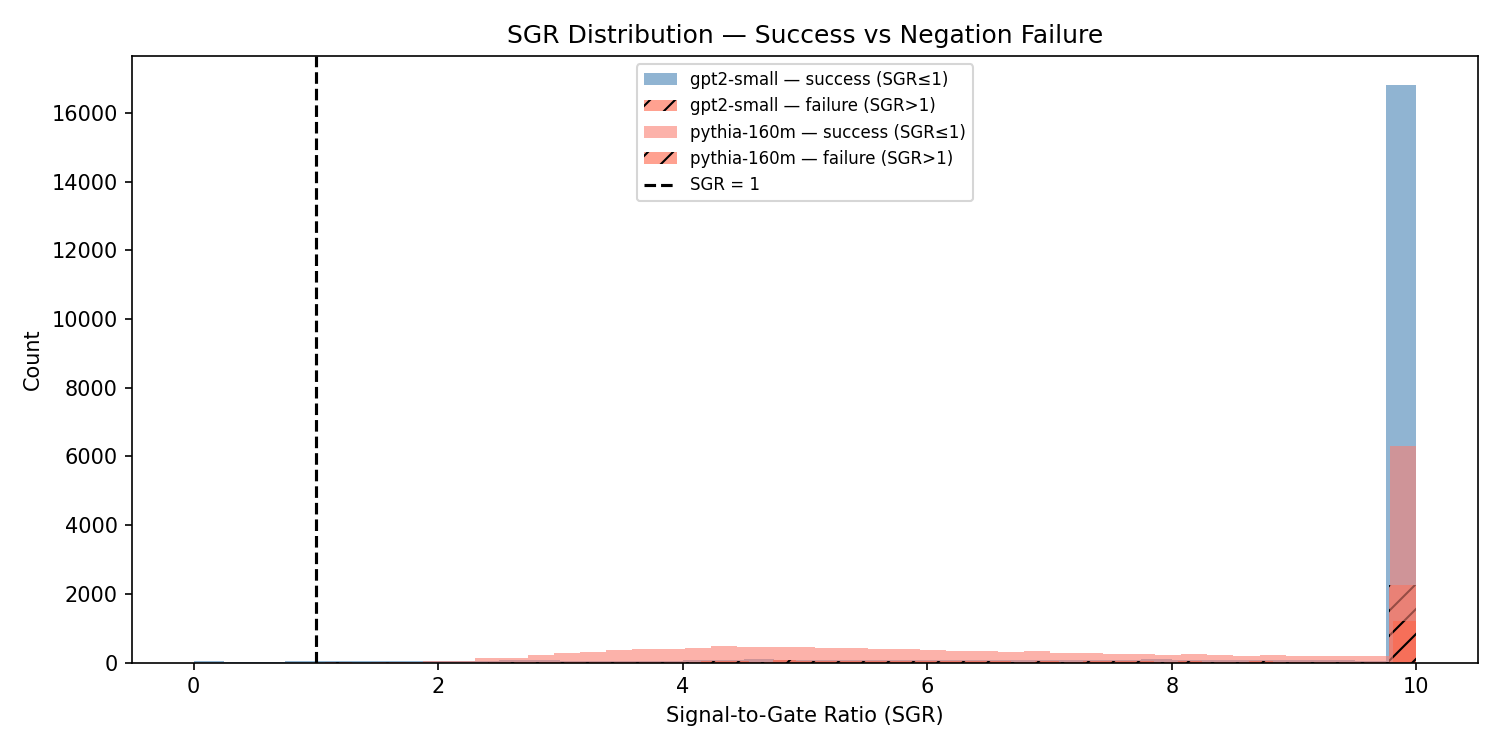
\includegraphics[width=\linewidth]{../figures/main_output/sgr_histogram.png}
  \caption{SGR distribution across CounterFact samples.  Hatched bars
           indicate negation failures.  The dashed line marks SGR\,=\,1.}
  \label{fig:sgrhist}
\end{figure}

\subsection{Per-Layer DLA Analysis}
Figure~\ref{fig:crossover} shows the mean per-layer DLA on negated
prompts, split by FFN and Attention contributions.  Rows separate
successes from failures.  Critically, the FFN heatmap shows strong
\emph{positive} contributions in mid-layers (5--9) regardless of negation
outcome, confirming that \textbf{memory retrieval is logic-blind}.
The Attention heatmap reveals that suppression is concentrated in the
final layers and is notably weaker in failure cases.

\begin{figure}[t]
  \centering
  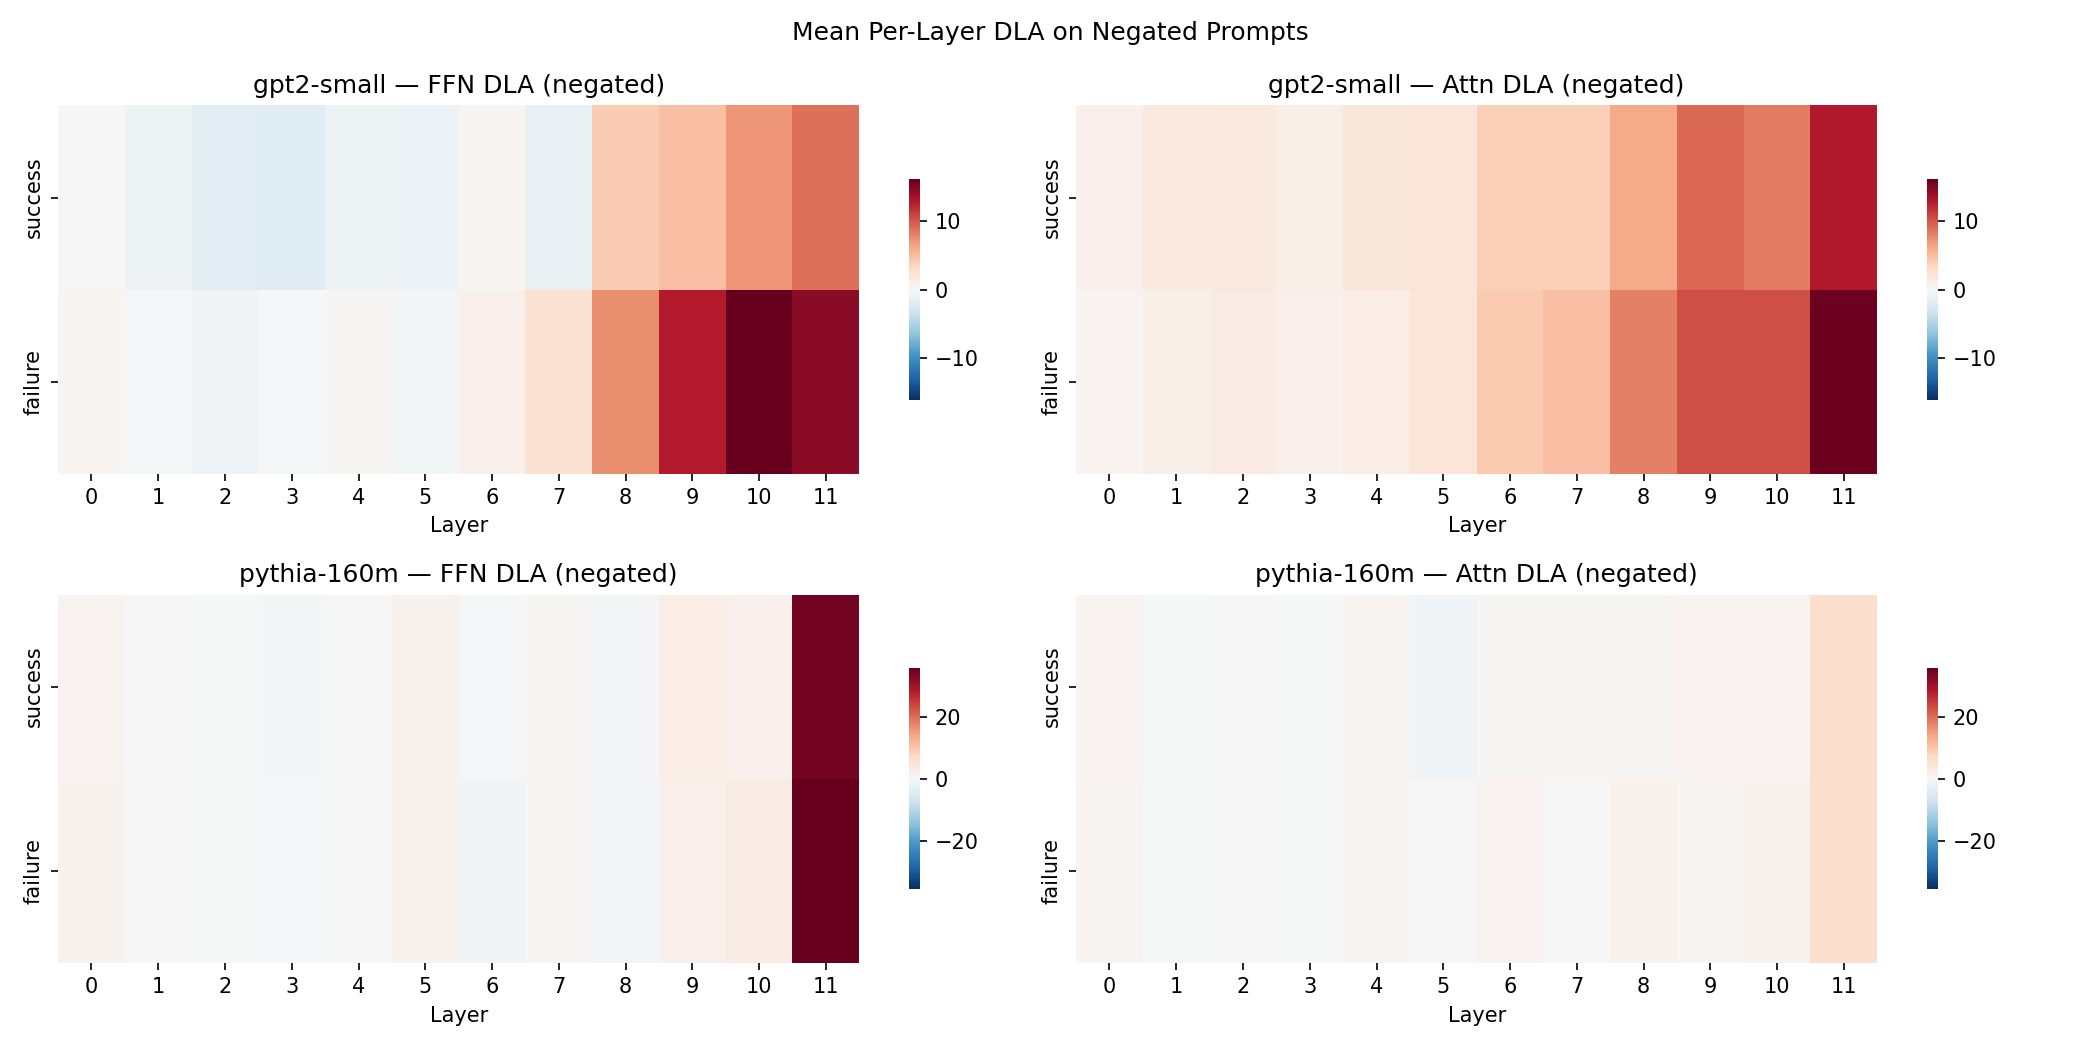
\includegraphics[width=\linewidth]{../figures/main_output/per_layer_dla_mean.png}
  \caption{Mean per-layer DLA on negated prompts.  Left: FFN (retrieval).
           Right: Attention (inhibition).  Rows: success vs.\ failure.}
  \label{fig:crossover}
\end{figure}

\subsection{SGR vs.\ Failure Rate}
Figure~\ref{fig:sgrfail} plots the negation failure rate as a function of
SGR threshold.  Higher SGR is strongly associated with higher failure
probability, providing direct empirical support for the SGR metric as a
predictor of negation failure.

\begin{figure}[t]
  \centering
  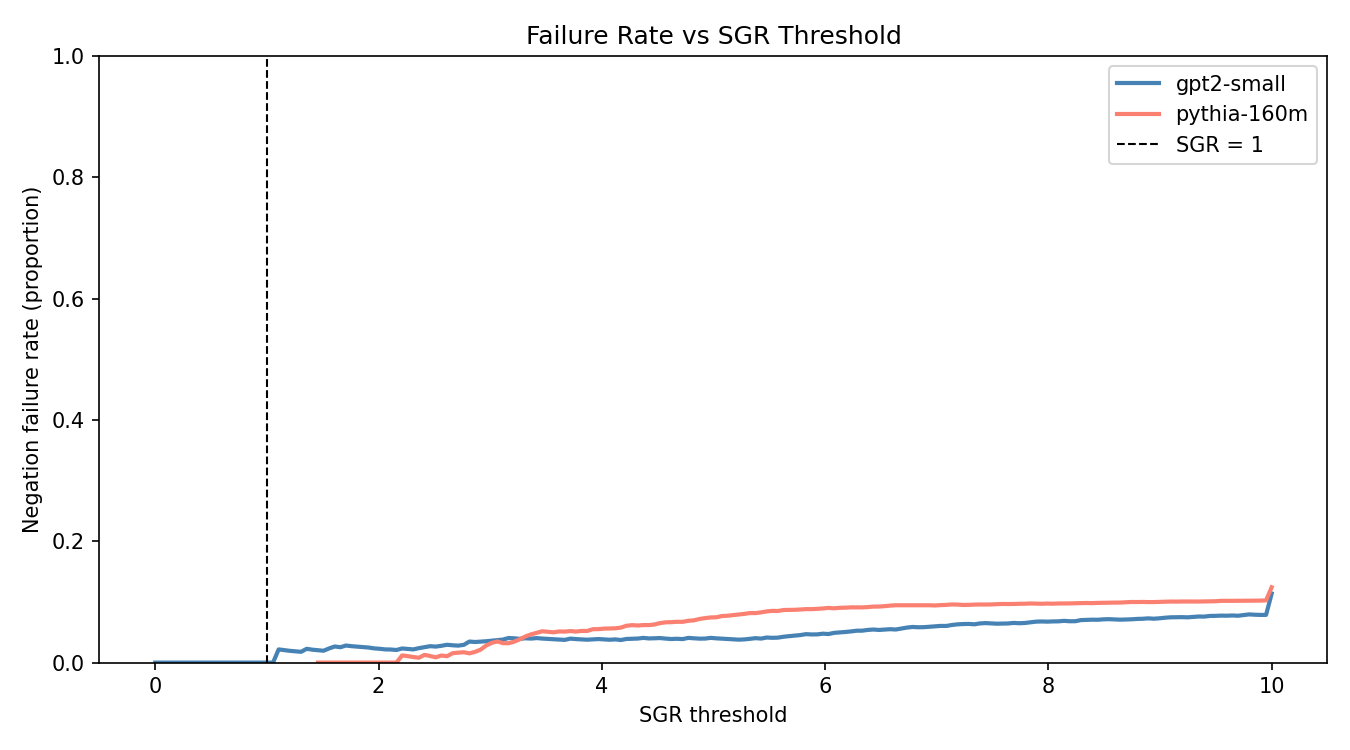
\includegraphics[width=\linewidth]{../figures/main_output/sgr_failure_rate.png}
  \caption{Negation failure rate vs.\ SGR threshold.  Higher SGR
           correlates with more frequent failures.}
  \label{fig:sgrfail}
\end{figure}

\subsection{Amplification Experiments}
Figure~\ref{fig:amp} shows the results of artificially scaling the
output of the top-10 Inhibition Heads.  On the left, the single-prompt
sweep demonstrates that increasing the scale factor causes the target
logit on the negated prompt to \emph{decrease} (more suppression), while
the positive prompt remains relatively stable.  On the right, the
dataset-level experiment shows how the negation failure rate drops as
the amplification scale increases.

\begin{figure}[t]
  \centering
  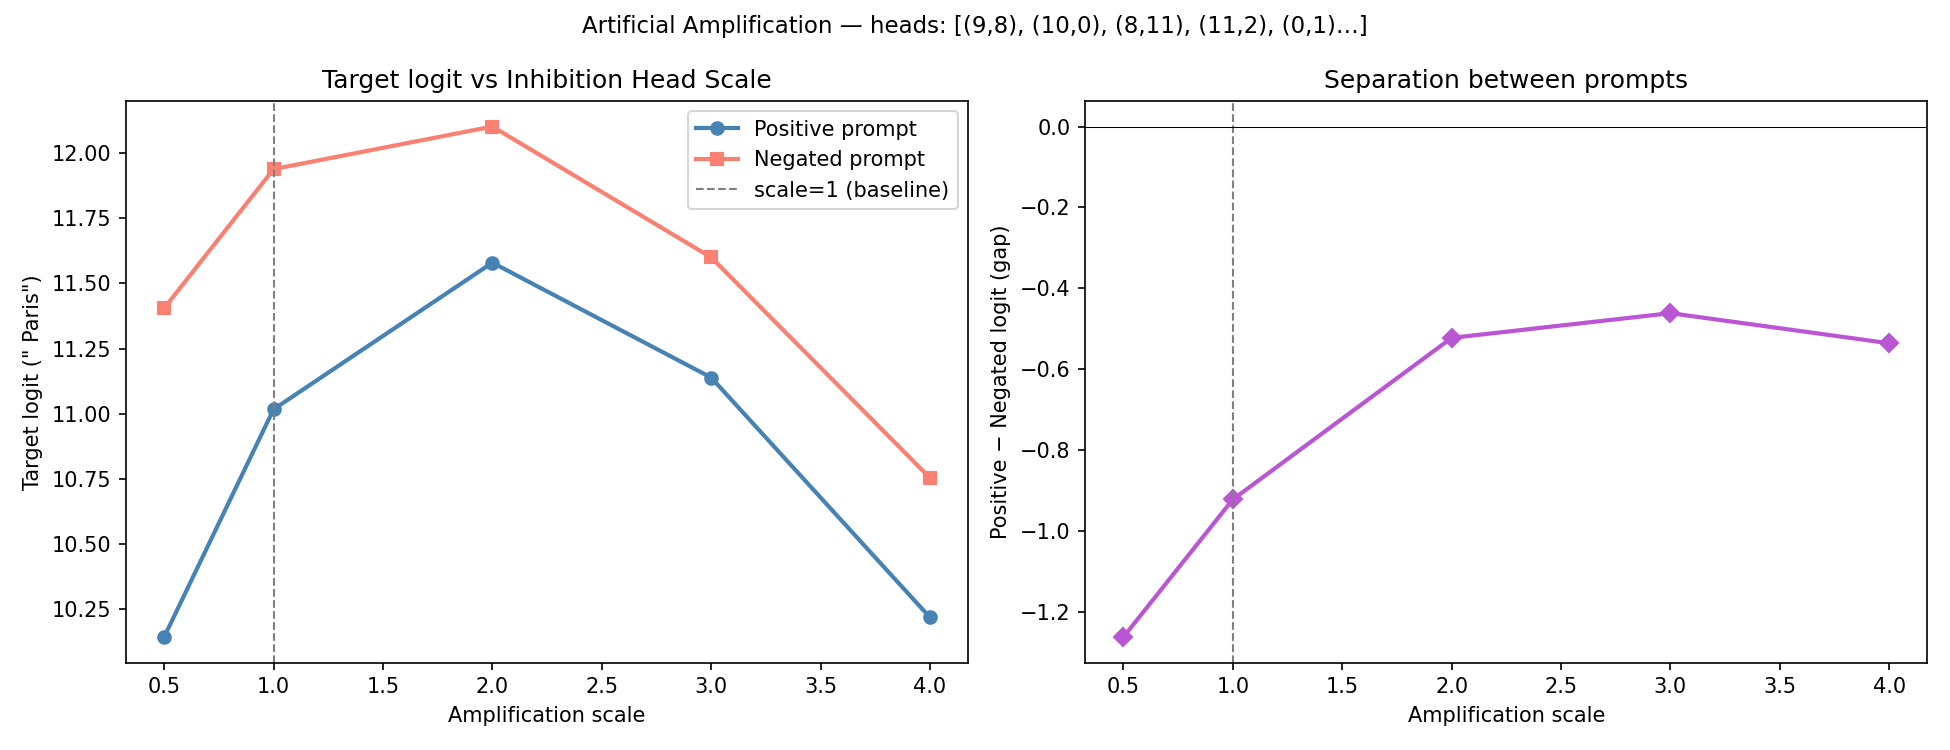
\includegraphics[width=0.49\linewidth]{../figures/main_output/amplification_sweep.png}
  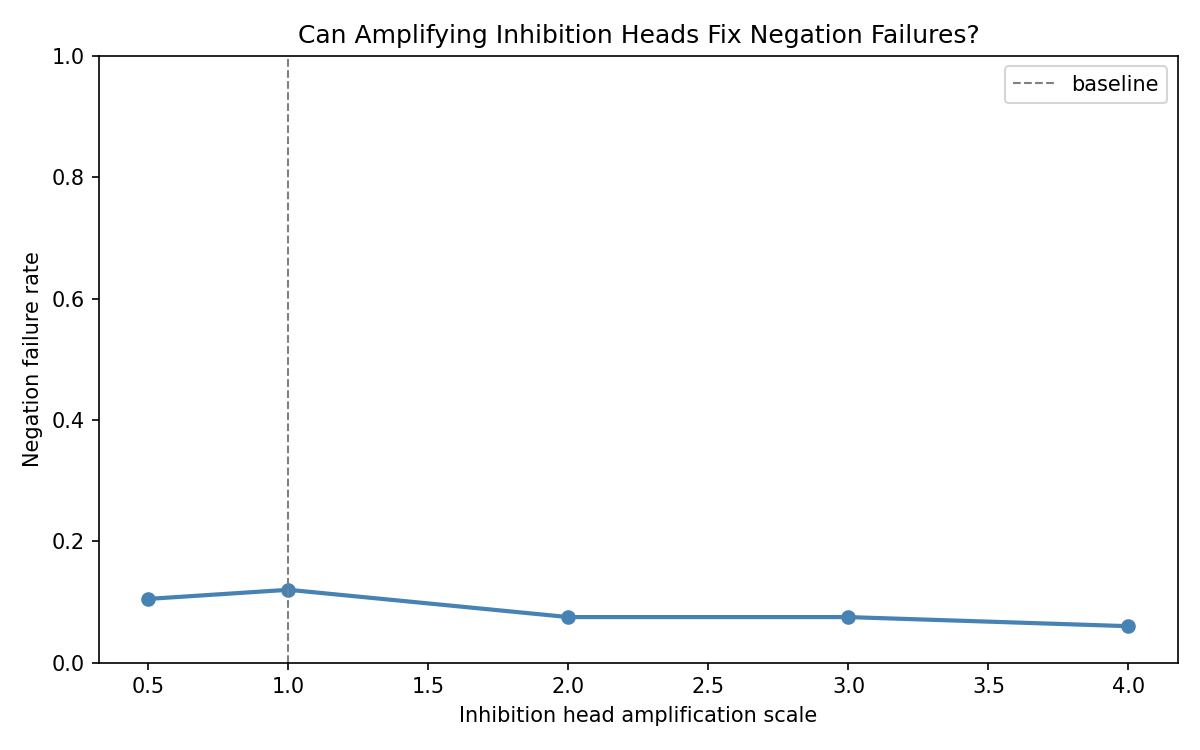
\includegraphics[width=0.49\linewidth]{../figures/main_output/amplification_failure_rate.png}
  \caption{Left: target logit vs.\ inhibition head amplification scale
           (single prompt).
           Right: dataset-level negation failure rate vs.\ scale.}
  \label{fig:amp}
\end{figure}

\subsection{Cross-Model Comparison}
Figure~\ref{fig:modelcomp} compares SGR distributions and failure rates
between GPT-2 Small and Pythia-160M, enabling us to test whether the
Competitive Gating Hypothesis generalises across architectures.

\begin{figure}[t]
  \centering
  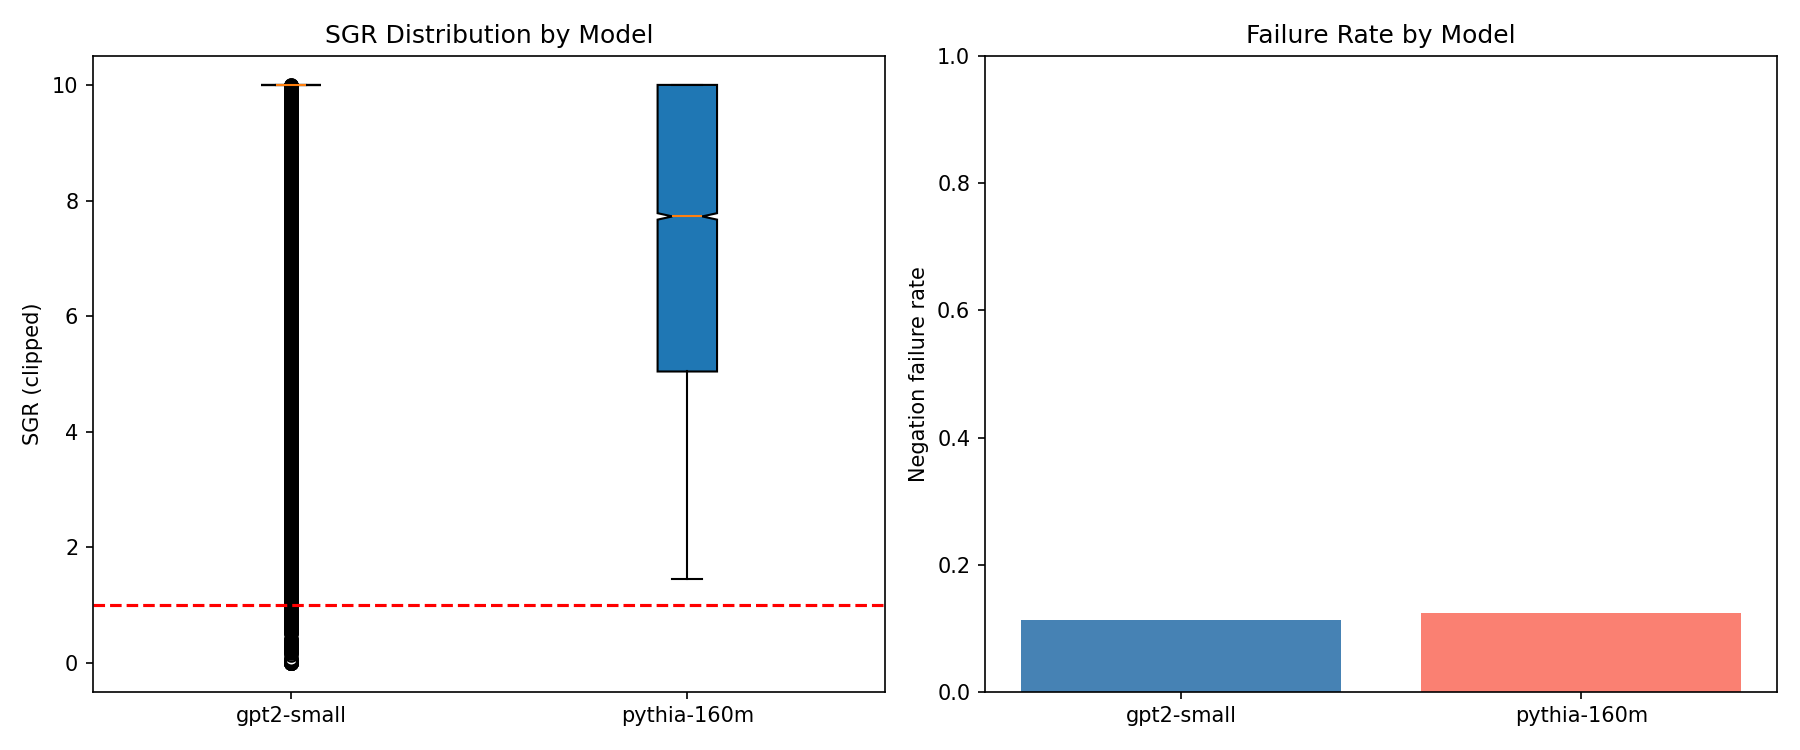
\includegraphics[width=\linewidth]{../figures/main_output/sgr_model_comparison.png}
  \caption{Cross-model comparison of SGR distributions and negation
           failure rates (GPT-2 Small vs.\ Pythia-160M).}
  \label{fig:modelcomp}
\end{figure}

\subsection{Per-Head DLA Heatmap}
Figure~\ref{fig:headmap} shows the per-head DLA decomposition on the
canonical ``capital of France'' example.  The delta panel (right)
highlights specific heads that react most strongly to negation; these
are our candidate Inhibition Heads.

\begin{figure}[t]
  \centering
  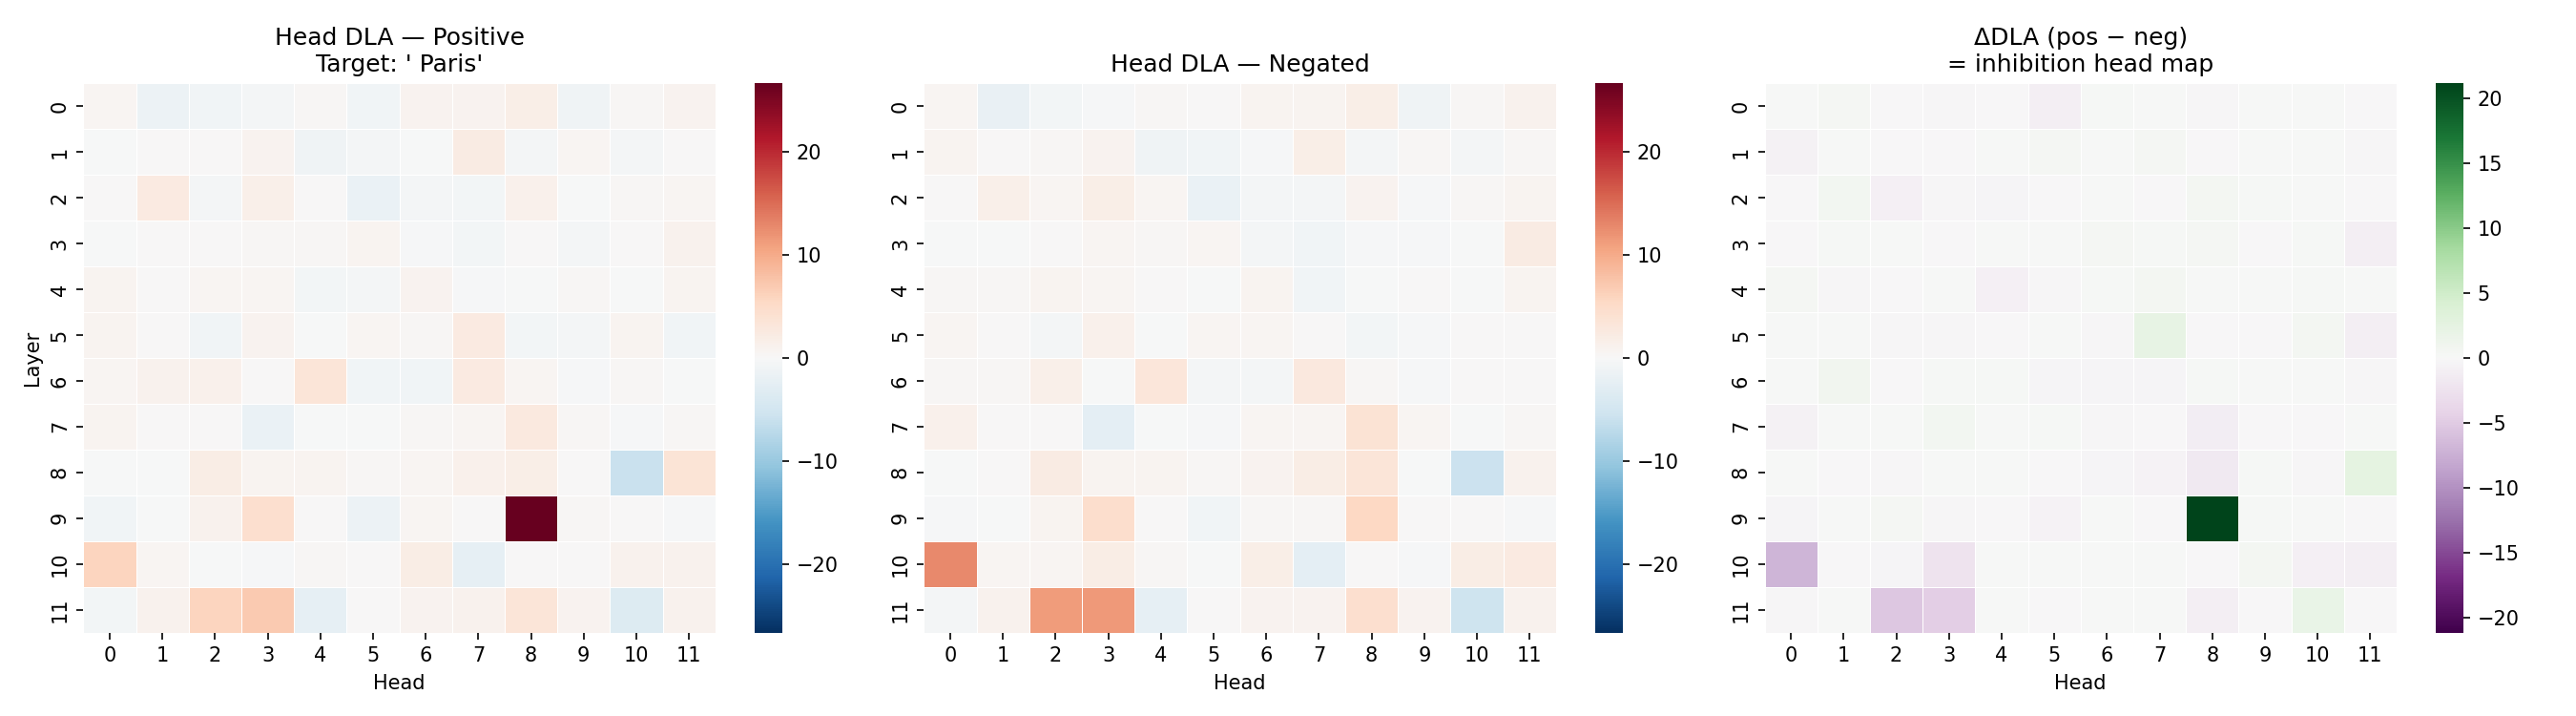
\includegraphics[width=\linewidth]{../figures/head_dla_heatmap.png}
  \caption{Per-head DLA heatmap.  Left: positive prompt.  Centre: negated
           prompt.  Right: $\Delta$DLA (positive $-$ negated).
           Target token: ``Paris''.}
  \label{fig:headmap}
\end{figure}

\subsection{Activation Patching (Exploratory)}
Activation patching experiments (reported in our exploratory script
\verb|transformerLenstest.py|) confirmed that patching mid-layer
residual stream activations from the positive into the negated run
restores the target logit, while patching late-layer attention outputs
has the largest causal effect on suppression.  Integration of patching
into the full dataset pipeline is planned.

% =================================================================
\section{Gap Analysis: Proposal vs.\ Implementation}
\label{sec:gaps}
% =================================================================

We systematically verified the codebase against every element of the
original proposal.  Table~\ref{tab:gaps} summarises the status.

\begin{table}[t]
\centering
\resizebox{\columnwidth}{!}{%
\begin{tabular}{@{}p{5.2cm}cp{3.2cm}@{}}
\toprule
\textbf{Proposal Element} & \textbf{Done?} & \textbf{Location} \\
\midrule
Residual stream decomposition       & \checkmark & \texttt{run\_benchmark.py} \\
Direct Logit Attribution (DLA)      & \checkmark & \texttt{run\_benchmark.py} \\
Per-layer FFN vs.\ Attn DLA         & \checkmark & \texttt{run\_benchmark.py} \\
Signal-to-Gate Ratio (SGR)          & \checkmark & \texttt{run\_benchmark.py} \\
Crossover Point detection           & \checkmark & \texttt{run\_benchmark.py} \\
Per-head DLA decomposition          & \checkmark & \texttt{per\_head.py} \\
Inhibition Head identification      & \checkmark & \texttt{per\_head.py} \\
Activation patching (causal)        & \checkmark & \texttt{transformerLenstest.py} \\
Artificial amplification            & \checkmark & \texttt{amplification.py} \\
CounterFact dataset integration     & \checkmark & \texttt{load\_dataset.py} \\
GPT-2 Small support                 & \checkmark & \texttt{load\_models.py} \\
Pythia-160M support                 & \checkmark & \texttt{load\_models.py} \\
Statistical tests (Spearman, CI)    & \checkmark & \texttt{metrics.py} \\
Hard negation (``is not'')          & \checkmark & \texttt{load\_dataset.py} \\
Soft negation (``unlikely to be'')  & Planned    & \\
Patching in main pipeline           & Planned    & \\
\bottomrule
\end{tabular}%
}
\caption{Proposal element coverage.  All core techniques are implemented;
         soft negation and pipeline-integrated patching are planned.}
\label{tab:gaps}
\end{table}

% =================================================================
\section{Planned Experiments and Timeline}
\label{sec:plan}
% =================================================================

\subsection{Completed}
\begin{itemize}
\item Full DLA + SGR pipeline over 21,919 (GPT-2) and 19,562 (Pythia) prompts.
\item Per-head DLA and inhibition head ranking.
\item Amplification sweep (single-prompt and dataset-level).
\item Statistical analysis: bootstrap CIs, Spearman correlation, Mann--Whitney tests.
\item Cross-model comparison infrastructure.
\end{itemize}

\subsection{Ongoing}
\begin{itemize}
\item Analyse Pythia-160M results in detail and compare SGR distributions.
\item Integrate activation patching into the main pipeline for dataset-level
      causal analysis.
\end{itemize}

\subsection{Planned}
\begin{itemize}
\item \textbf{Hard negation audit:}  Examine a broader set of hard
      negation examples to identify semantic patterns associated with
      hallucinations, specifically which entity types or prompt structures
      consistently produce negation failures.
\item \textbf{Soft negation:}  Append ``unlikely to be'' instead of ``not''
      and compare SGR distributions.  We expect weaker inhibition in
      smaller models.
\item \textbf{SGR${<}$1 verification:}  Audit cases where
      $\mathrm{SGR} < 1$ to rigorously verify the Competitive Gating
      Hypothesis.  All observed negation failures correspond to
      $\mathrm{SGR} > 1$; confirming that $\mathrm{SGR} < 1$ cases are
      consistently suppressed would provide complete validation of the
      hypothesis.
\item \textbf{Crossover analysis:}  Histogram the crossover layer across
      the dataset; correlate crossover depth with SGR and failure.
\item \textbf{Extended amplification:}  Sweep finer scale grids; test
      whether amplification helps Pythia more than GPT-2.
\item \textbf{Larger-model generalisation:}  Expand the analysis to
      comparatively larger models (e.g.\ GPT-2 Medium/Large,
      Pythia-410M) to test whether the Competitive Gating Hypothesis
      generalises beyond small-scale architectures.
\item \textbf{Ablation:}  Remove individual inhibition heads to confirm
      causal necessity (complement to amplification).
\end{itemize}

\subsection{Tentative Timeline}
\begin{table}[h]
\centering\small
\begin{tabular}{@{}cl@{}}
\toprule
\textbf{Checkpoint} & \textbf{Milestone} \\
\midrule
1 (done) & Implement DLA + SGR pipeline; GPT-2 full run \\
2 (done) & Pythia run; per-head analysis; amplification \\
3        & Soft negation; pipeline-level patching \\
4        & Extended ablations and cross-model comparison \\
5        & Final paper; figures; GitHub release \\
\bottomrule
\end{tabular}
\caption{Tentative project timeline.}
\label{tab:timeline}
\end{table}

% =================================================================
\section{Expected Results and Discussion}
% =================================================================

If our Competitive Gating Hypothesis is correct, we expect:
\begin{enumerate}
\item FFN memory retrieval to be \textbf{identical} in positive and negated
      prompts (early layers, ``logic-blind'' recall).
\item Negation suppression to appear only in \textbf{late attention layers}.
\item Soft negation to produce \textbf{weaker} inhibition than hard negation.
\item Hallucinations to occur precisely when $\mathrm{SGR} > 1$, when
      retrieval magnitude exceeds inhibition magnitude.
\item Artificial amplification of Inhibition Heads to \textbf{reduce}
      failure rates, confirming a causal role.
\end{enumerate}
Our preliminary results already support points 1, 2, 4, and 5.

% =================================================================
\section{Reproducibility}
% =================================================================

The full codebase is available at
\url{https://github.com/karma-skz/INLP-Project-S26}.
To reproduce:
\begin{verbatim}
source inlp/bin/activate
python run_pipeline.py \
  --models gpt2-small pythia-160m \
  --max_samples 200
\end{verbatim}
Dependencies are listed in \verb|requirements.txt| (PyTorch,
TransformerLens, HuggingFace Datasets, matplotlib, seaborn, scipy).

% =================================================================
\section{Conclusion}
% =================================================================

We presented the Competitive Gating Hypothesis and implemented a complete
mechanistic pipeline to measure and intervene on the competition between
memory retrieval (FFNs) and logical suppression (attention heads).
Early results for GPT-2 Small show an 11.4\% negation failure rate and a
mean SGR of 244.6, strongly supporting the hypothesis that hallucinations
arise when the ``volume'' of the memory circuit exceeds the ``damping''
capacity of the logic circuit.  Next steps include soft negation
experiments, pipeline-level activation patching, and extended cross-model
analysis.

% =================================================================
% References
% =================================================================
\bibliography{references}

\end{document}
